\documentclass{article}
\usepackage[english,greek, main=greek]{babel}
\usepackage[utf8]{inputenc}
\usepackage{fullpage}
\usepackage{amsmath} 
\usepackage{graphicx} % for graphics and plots
\usepackage{subcaption} % for subfigures and subcaptions and \ContinuedFloat
\usepackage{placeins} % for \FloatBarrier
\usepackage{xcolor} % for colour definitions
\usepackage{listings} % for code highlighting
\usepackage{verbatim} % for file input
\usepackage{hyperref} % clickable links
\usepackage[explicit]{titlesec} % number after section name
\titleformat{\section}  % avoid numbering the table of contents
  {\normalfont\Large\bfseries}
  {}
  {0em}
  {\ifnum\value{section}=0\relax #1\else #1\ \thesection\fi}

\newcommand{\eng}[1]{\foreignlanguage{english}{#1}} % shortcut for inserting english into greek text

\useshorthands{;}
\defineshorthand{;}{?} % greek question mark instead of english semicolon

\definecolor{mGreen}{rgb}{0,0.6,0}
\definecolor{mGray}{rgb}{0.5,0.5,0.5}
\definecolor{mPurple}{rgb}{0.58,0,0.82}
\definecolor{light-gray}{gray}{0.95}
\definecolor{backgroundColour}{rgb}{0.95,0.95,0.92}

\lstdefinestyle{CStyle}{
    backgroundcolor=\color{backgroundColour},   
    commentstyle=\color{mGreen},
    keywordstyle=\color{magenta},
    numberstyle=\tiny\color{mGray},
    stringstyle=\color{mPurple},
    basicstyle=\footnotesize,
    breakatwhitespace=false,         
    breaklines=true,                 
    keepspaces=true,                 
    numbers=left,                    
    numbersep=5pt,                  
    showspaces=false,                
    showstringspaces=false,
    showtabs=false,                  
    tabsize=2,
    language=C
}

\lstset{language=bash, 
    basicstyle=\small\ttfamily, 
    keywordstyle=\color{blue}\bfseries, 
    commentstyle=\color{gray}, 
    stringstyle=\color{green!50!black},
    backgroundcolor=\color{light-gray},
    showstringspaces=false,
    breaklines=true,
    linewidth=\textwidth}

\title{
    \includegraphics[width=\textwidth]{~/Pictures/emp.png} \\
    \vskip 5cm
    Σχεδιασμός Ενσωματωμένων Συστήματων \\
    \large Άσκηση 2η
    \vskip 5cm
}

\author{
    Αναστάσιος Στέφανος Αναγνώστου \\ \large 03119051 \and
    Σαββίνα Νάστου \\ \large 03119146
}

\begin{document}

\maketitle \clearpage \tableofcontents \clearpage

\section{Ζητούμενο}

\subsection{}

Η εκτέλεση της εφαρμογής για όλους τους διαφορετικούς
συνδυασμοςύ υλοποιήσεων δομών δεδομένων και η αντίστοιχη
καταγραφή των προσβάσεων στην μνήμη και της απαιτούμενης
μνήμης έγινε χρήσει του \eng{script} \ref{lst:run-drr}.

\begin{figure}[h]
    \begin{subfigure}{0.4\textwidth}
        \selectlanguage{english}
        \verbatiminput{../src/DRR/mem_accesses_labeled.txt}
        \selectlanguage{greek}
    \end{subfigure}
    \begin{subfigure}{0.6\textwidth}
        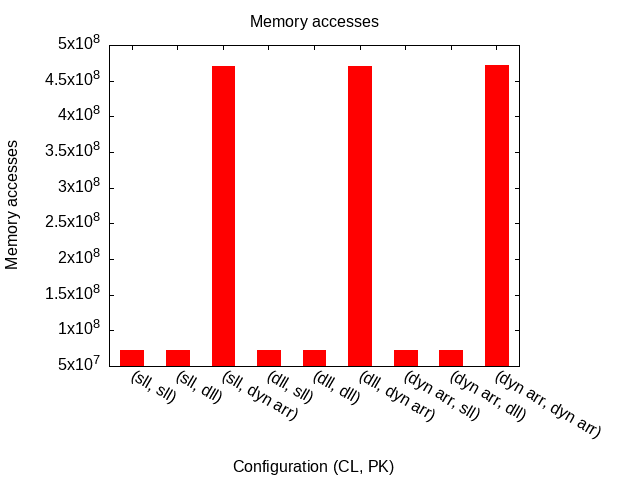
\includegraphics[width=\textwidth]{../src/DRR/mem_accesses.png}
    \end{subfigure}
    \caption{Προσβάσεις στην μνήμη ανά συνδυασμό δομών}
    \begin{subfigure}{0.4\textwidth}
        \selectlanguage{english}
        \verbatiminput{../src/DRR/mem_footprints_labeled.txt}
        \selectlanguage{greek}
    \end{subfigure}
    \begin{subfigure}{0.6\textwidth}
        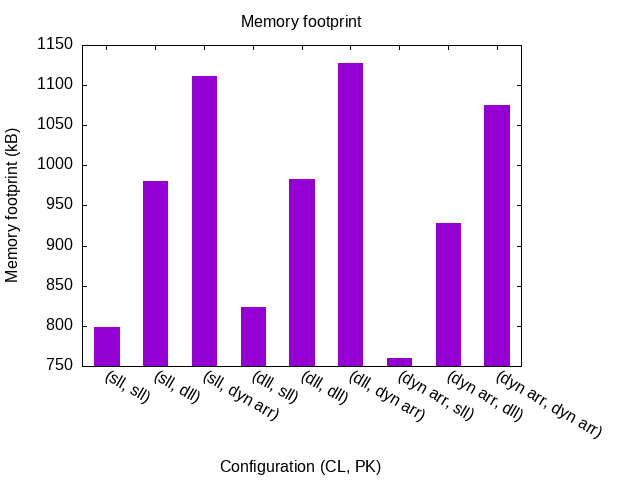
\includegraphics[width=\textwidth]{../src/DRR/mem_footprint.png}
    \end{subfigure}
    \caption{Απαίτηση μνήμης (ΚΒ) ανά συνδυασμό δομών}
\end{figure}
\FloatBarrier

\subsection{}

\subsection{}

\clearpage
\section{Ζητούμενο}

\subsection{}

Η έξοδος του προγράμματος είναι:

\begin{figure}[h]
    \centering
    \selectlanguage{english}
    \verbatiminput{../src/dijsktra/paths.out}
    \selectlanguage{greek}
\end{figure}

\subsection{}

Οι αλλαγές στον κώδικα φαίνονται στο αρχείο \ref{lst:dijkstra}.

\subsection{}

Οι εκτελέσεις των διάφορων παραλλαγών έγιναν χρήσει του \eng{script}
\ref{lst:run-dijkstra}. Ανά εκτέλεση ελεγχόταν η έξοδος ώστε να 
επικυρώνεται η ορθότητα του προγράμματος.

\begin{figure}[h]
    \begin{subfigure}{0.4\textwidth}
        \selectlanguage{english}
        \verbatiminput{../src/dijsktra/mem_accesses_labeled.txt}
        \selectlanguage{greek}
    \end{subfigure}
    \begin{subfigure}{0.6\textwidth}
        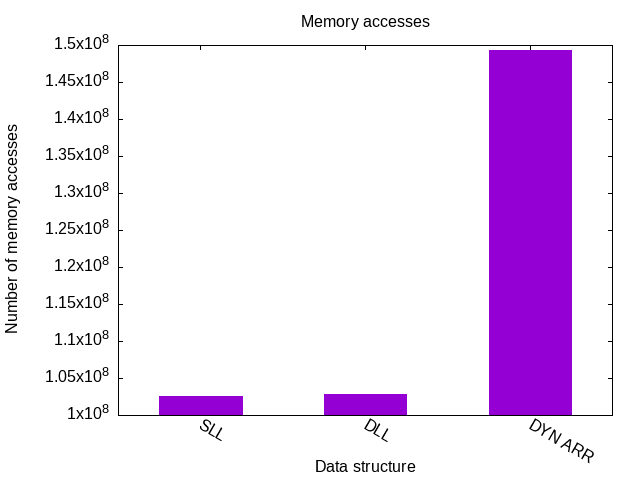
\includegraphics[width=\textwidth]{../src/dijsktra/mem_access.png}
    \end{subfigure}
    \caption{Προσβάσεις στην μνήμη ανά δομή}
    \begin{subfigure}{0.4\textwidth}
        \selectlanguage{english}
        \verbatiminput{../src/dijsktra/mem_footprints_labeled.txt}
        \selectlanguage{greek}
    \end{subfigure}
    \begin{subfigure}{0.6\textwidth}
        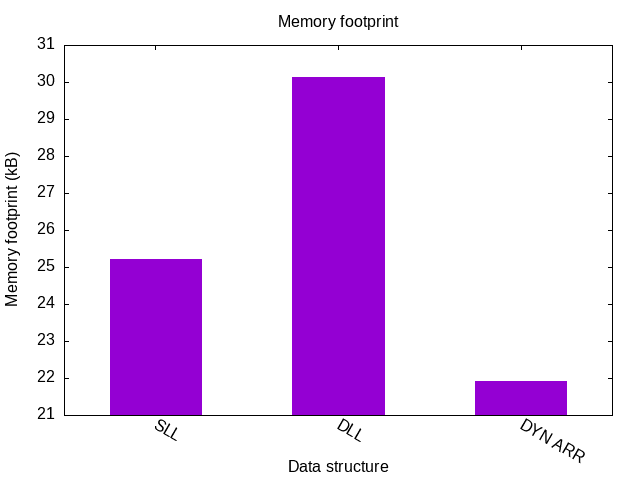
\includegraphics[width=\textwidth]{../src/dijsktra/mem_footprint.png}
    \end{subfigure}
    \caption{Απαίτηση μνήμης (ΚΒ) ανά δομή}
\end{figure}
\FloatBarrier

\subsection{}

\subsection{}

\clearpage
\section*{Παράρτημα}

\selectlanguage{english}
\lstinputlisting[caption={run-drr.sh}, label={lst:run-drr}]{../src/DRR/run_experiments_drr.sh}
\clearpage
\lstinputlisting[caption={dijkstra.c}, label={lst:dijkstra}]{../src/dijsktra/dijkstra.c}
\clearpage
\lstinputlisting[caption={run-dijkstra.sh}, label={lst:run-dijkstra}]{../src/dijsktra/run_experiments_dijkstra.sh}



\end{document}
